% ==============================================================================
% CHAPITRE 3 : ARCHITECTURE SYSTÈME ET MODÈLE DE DONNÉES
% ==============================================================================

\chapter{Architecture Système et Modèle de Données}
\label{ch:architecture}

\section{Exigences du cahier des charges}

Le cahier des charges du Mini-Projet 17 impose dix exigences techniques et opérationnelles résumées dans le Tableau~\ref{tab:business_requirements}.

\begin{table}[htbp]
\centering
\caption{Synthèse des exigences fonctionnelles du projet}
\label{tab:business_requirements}
\footnotesize
\begin{tabularx}{\textwidth}{l p{4.2cm} X}
\toprule
\textbf{Réf.} & \textbf{Intitulé de l'Exigence} & \textbf{Implémentation dans notre Système} \\
\midrule
\textbf{BR-01} & Ingestion continue & Connecteur Spark Structured Streaming consommant le topic Kafka \texttt{financial-transactions}. \\
\textbf{BR-02} & Graphe orienté dynamique & Projection en mémoire des comptes ($V$) et des transferts ($E$) sous forme de DataFrames. \\
\textbf{BR-03} & Cycles d'ordre 3 ($k=3$) & Requête de motif GraphFrames extrayant les boucles $A \to B \to C \to A$. \\
\textbf{BR-04} & Fenêtrage temporel & Fenêtres glissantes de $10\text{ min}$ (pas de $30\text{ s}$) et watermark de $120\text{ s}$. \\
\textbf{BR-05} & Métriques de graphe & Recalcul périodique (toutes les $60\text{ s}$) du PageRank et des composantes connexes. \\
\textbf{BR-06} & Diffusion des alertes & Publication en temps réel des alertes de fraude sur le topic Kafka dédié \texttt{fraud-alerts}. \\
\textbf{BR-07} & Stockage Lakehouse ACID & Sauvegarde continue dans Delta Lake avec déduplication par hachage canonique. \\
\textbf{BR-08} & Interface d'investigation & Cockpit web développé en Next.js 14 avec affichage vectoriel des cycles et export SAR. \\
\textbf{BR-09} & Points d'entrée unifiés CLI & 4 scripts Python standardisés : producteur, moteur de streaming, schémas, dashboard. \\
\textbf{BR-10} & Latence sub-seconde & Optimisation des micro-lots pour un temps de traitement moyen inférieur à $50\text{ ms}$. \\
\bottomrule
\end{tabularx}
\end{table}

\section{Format canonique des transactions}

Chaque événement transactionnel émis par le producteur respecte un schéma JSON strict (version 1) :

\begin{lstlisting}[language=JSON, caption={Structure d'un événement de transaction financière}, label={lst:canonical_json}]
{
  "schema_version": 1,
  "transaction_id": "TXN-64CAB8C7BF32",
  "source_account": "ACC-0081",
  "target_account": "ACC-0014",
  "montant": 161232.57,
  "devise": "MAD",
  "type_operation": "VIREMENT",
  "timestamp": "2026-11-02T19:08:15Z"
}
\end{lstlisting}

\section{Mécanisme du fenêtrage temporel glissant}

Le moteur de streaming découpe le flux continu en fenêtres temporelles semi-ouvertes de durée $L = 600\text{ s}$ ($10\text{ minutes}$) glissant avec un pas $S = 30\text{ secondes}$ :
\begin{equation}
    \mathcal{W}_k = \left[ k \cdot 30\text{ s}, \; k \cdot 30\text{ s} + 600\text{ s} \right), \quad k \in \mathbb{Z}
\end{equation}

Une transaction horodatée à l'instant $t$ satisfait l'appartenance à $\mathcal{W}_k$ si et seulement si :
\begin{equation}
    k \cdot 30 \le t < k \cdot 30 + 600 \iff \left\lfloor \frac{t - 600}{30} \right\rfloor + 1 \le k \le \left\lfloor \frac{t}{30} \right\rfloor
\end{equation}

Le nombre de fenêtres actives englobant simultanément un même événement est strictement constant :
\begin{equation}
    N_{fenetres} = \frac{L}{S} = \frac{600\text{ s}}{30\text{ s}} = 20\text{ fenêtres glissantes}
\end{equation}
Cette imbrication implique qu'un cycle de fraude sera détecté par Spark dans 20 micro-fenêtres consécutives. Pour éviter d'inonder les analystes de 20 alertes identiques, le système calcule un identifiant d'alerte canonique unique et applique une écriture idempotente dans Delta Lake (critère AT-08).

\section{Cartographie des micro-services Docker Compose}

L'ensemble de l'infrastructure est déployé sous la forme de conteneurs Docker orchestrés par un fichier \texttt{docker-compose.yml} unifié :

\begin{figure}[htbp]
    \centering
    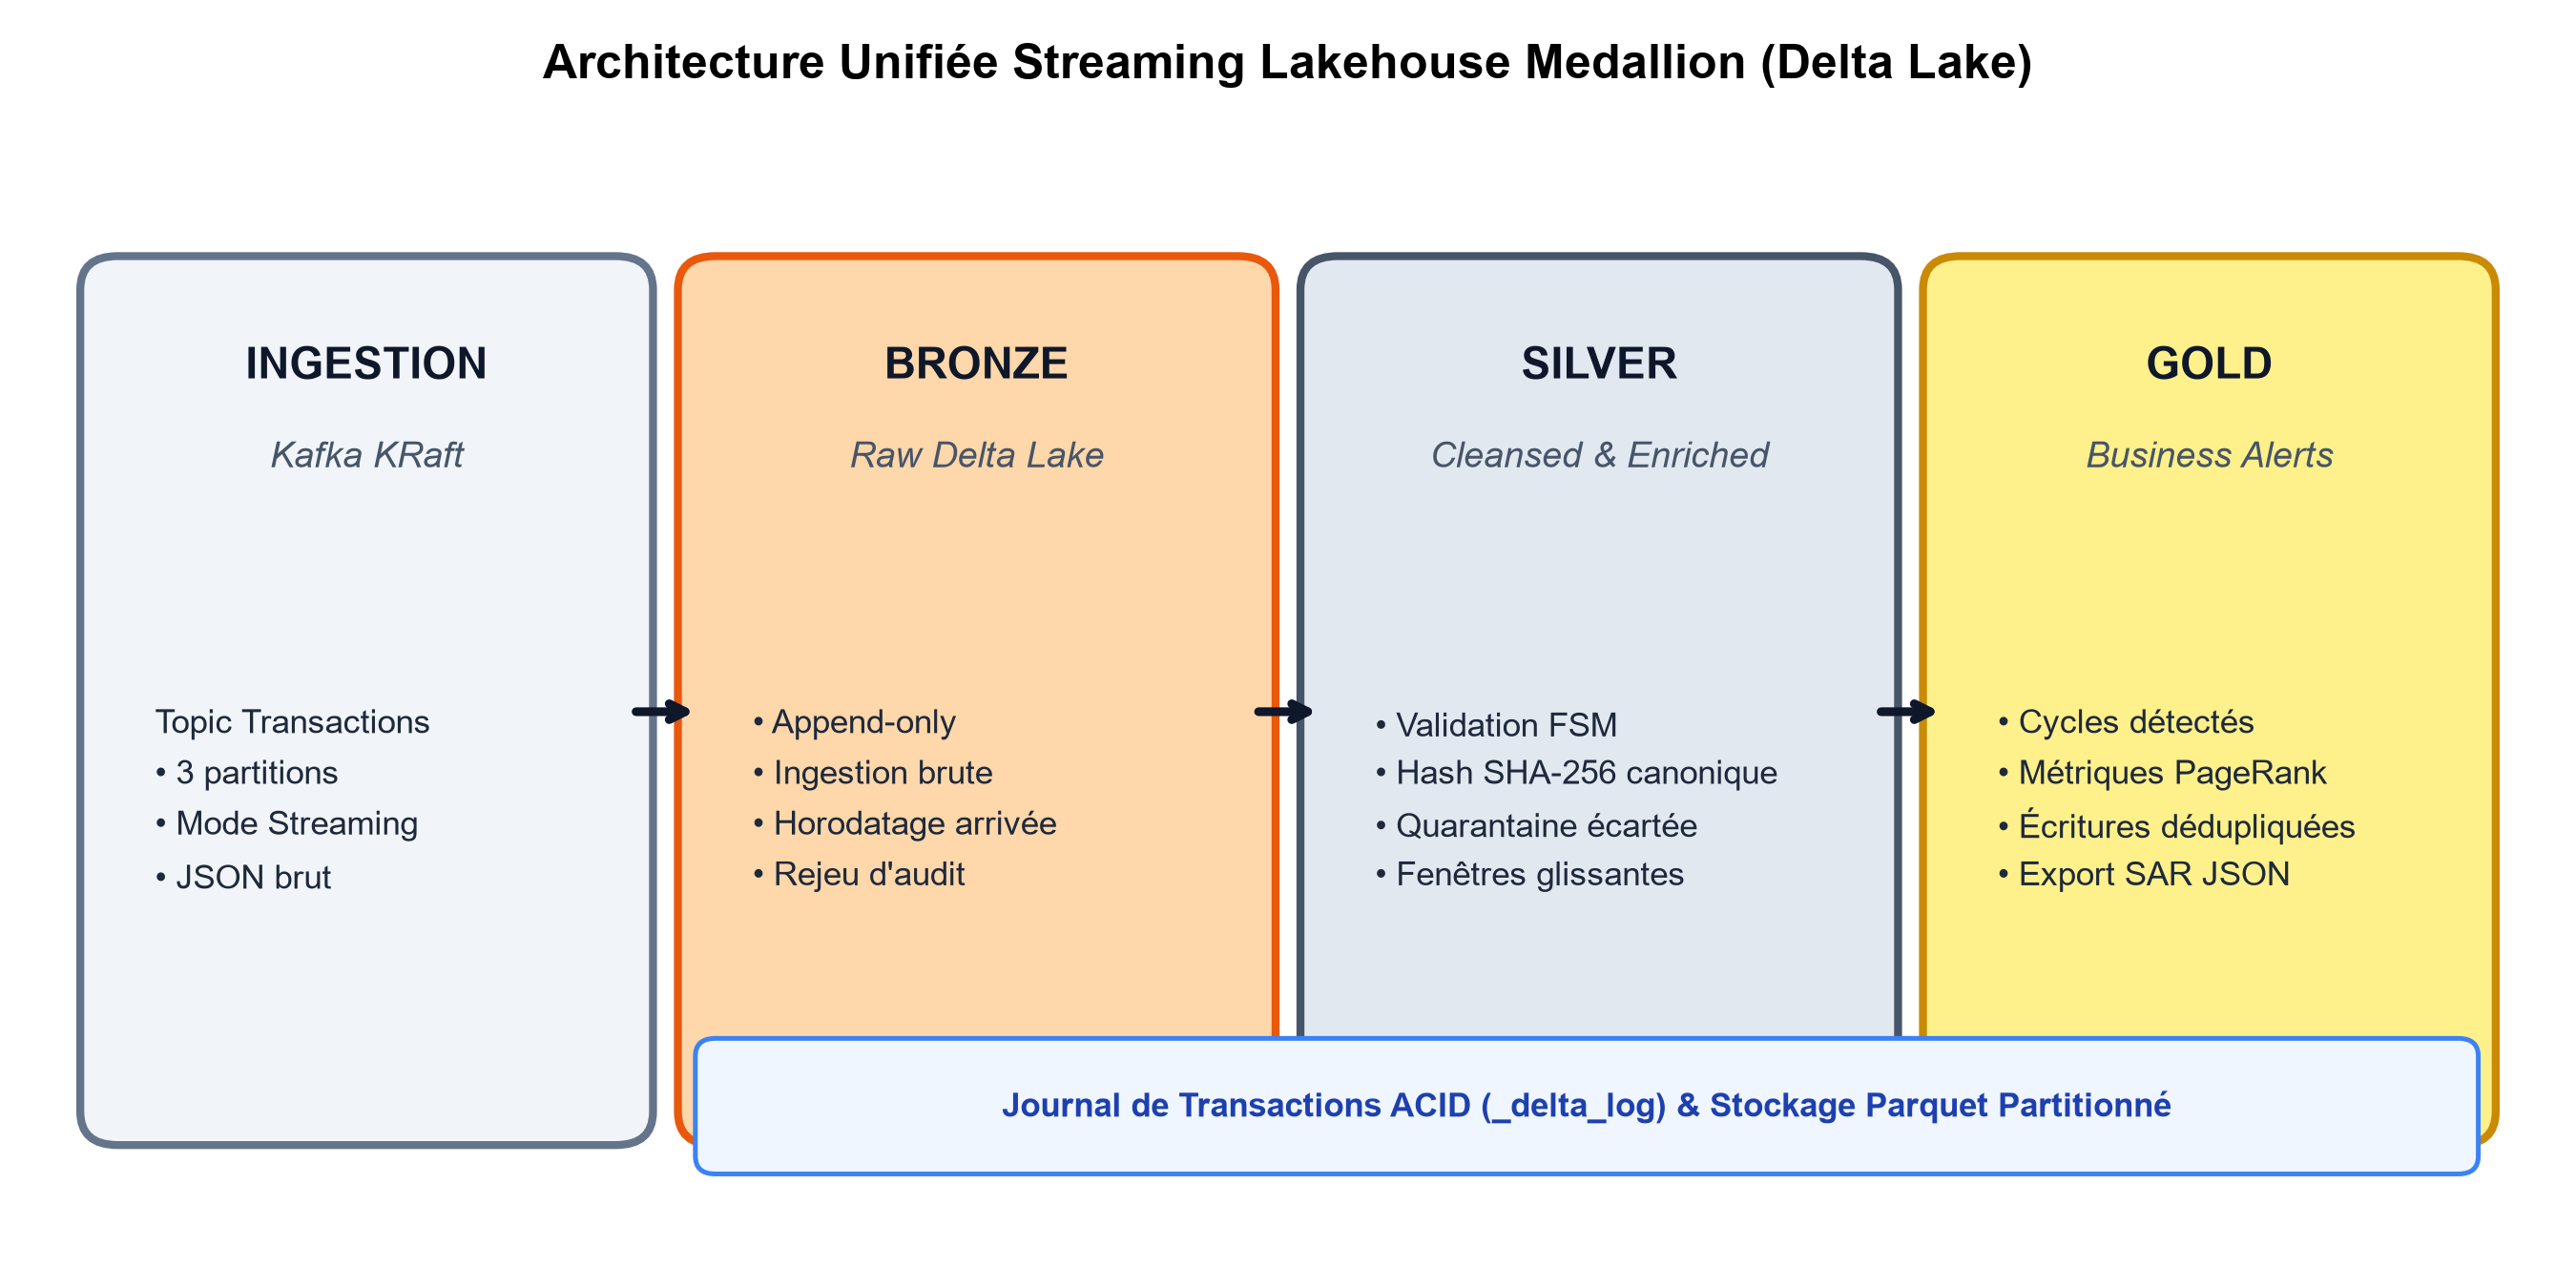
\includegraphics[width=0.92\linewidth]{figures/fig_lakehouse_architecture.png}
    \caption{Cartographie des micro-services Docker Compose et des flux de données distribués}
    \label{fig:docker_services_map}
\end{figure}

\begin{enumerate}
    \item \textbf{\texttt{aml-kafka} :} Broker Apache Kafka 3.5 en mode KRaft (consensus interne sans ZooKeeper), ports 9092 (inter-conteneurs) et 9094 (accès hôte) ;
    \item \textbf{\texttt{aml-kafka-ui} :} Console web de visualisation des messages et du débit des topics (port 8090) ;
    \item \textbf{\texttt{aml-spark-master} \& \texttt{aml-spark-worker} :} Cluster Spark 3.5.1 alloué à 4 cœurs CPU et 4 Go de mémoire RAM (ports 8080 et 8081) ;
    \item \textbf{\texttt{aml-spark-app} :} Conteneur d'exécution du pilote PySpark exécutant la boucle de détection GraphFrames ;
    \item \textbf{\texttt{aml-dashboard} :} Serveur d'application Next.js 14 servant l'interface analyste en temps réel (port 3000) ;
    \item \textbf{Volume persistant \texttt{delta-data} :} Volume partagé stockant les fichiers Parquet et le journal de logs ACID Delta Lake.
\end{enumerate}

\section{Structure des tables Delta Lake (Médaillon et Quarantaine)}

Pour garantir la traçabilité complète de chaque transaction, le stockage est organisé en dix tables Delta :
\begin{itemize}
    \item \textbf{\texttt{bronze\_transactions} :} Journal brut de toutes les charges utiles ingérées depuis Kafka ;
    \item \textbf{\texttt{silver\_transactions} :} Transactions sémantiquement validées et dédupliquées, prêtes pour l'analyse de graphe ;
    \item \textbf{\texttt{fraud\_alerts} :} Alertes confirmées de boucles de blanchiment avec montants, comptes et preuve JSON ;
    \item \textbf{Tables de rejet en quarantaine :} \texttt{quarantined\_transactions} (rejets schéma/montant), \texttt{duplicate\_transactions} (doublons), \texttt{conflict\_transactions} (conflits d'ID), et \texttt{late\_transactions} (retards hors filigrane) ;
    \item \textbf{Tables de métriques :} \texttt{account\_metrics} (scores PageRank) et \texttt{graph\_analytics\_metrics} (latence et taille du graphe).
\end{itemize}
